\subsection{Alternative Splicing}

L'Alternative Splicing è un metodo utilizzato dalle cellule per produrre proteine diverse dallo stesso frammento di DNA che viene utilizzato da oltre il 75\% dei geni umani. 

Considerando un generico locus, esso può essere diviso in esoni (parti codificanti) e introni (parti non codificanti). Durante la fase di Trascrizione gli introni vengono rimossi e la Timina viene trasformata in Uracile, ottenendo pre-RNA. A questo punto, in un normale processo di Splicing, tutti gli esoni vengono utilizzati, nell'ordine in cui appaiono nel pre-RNA, per ottenere una proteina. Nel caso di un evento di Alternative Splicing, questo non accade: alcuni esoni potrebbero infatti non essere utilizzati, o apparire in un ordine diverso. 

Vengono riconosciuti 5 tipi di eventi di Alternative Splicing:

\begin{enumerate}
	\item \textbf{Exon Skipping}: Almeno un esone non appare nel trascritto
	\item \textbf{Mutually Exclusive Exons}: Almeno due esoni non compaiono mai in uno stesso trascritto
	\item \textbf{Alternative 5' Donor Site}: Parte di un introne nel 5' diventa un esone
	\item \textbf{Alternative 3' Acceptor Site}: Parte di un introne nel 3' diventa un esone
	\item \textbf{Intron Retention}: Parte di un esono diventa un introne
\end{enumerate}

ASGAL è in grado di rilevarli tutti tranne il caso 2.

\begin{figure}[h]
	\centering
	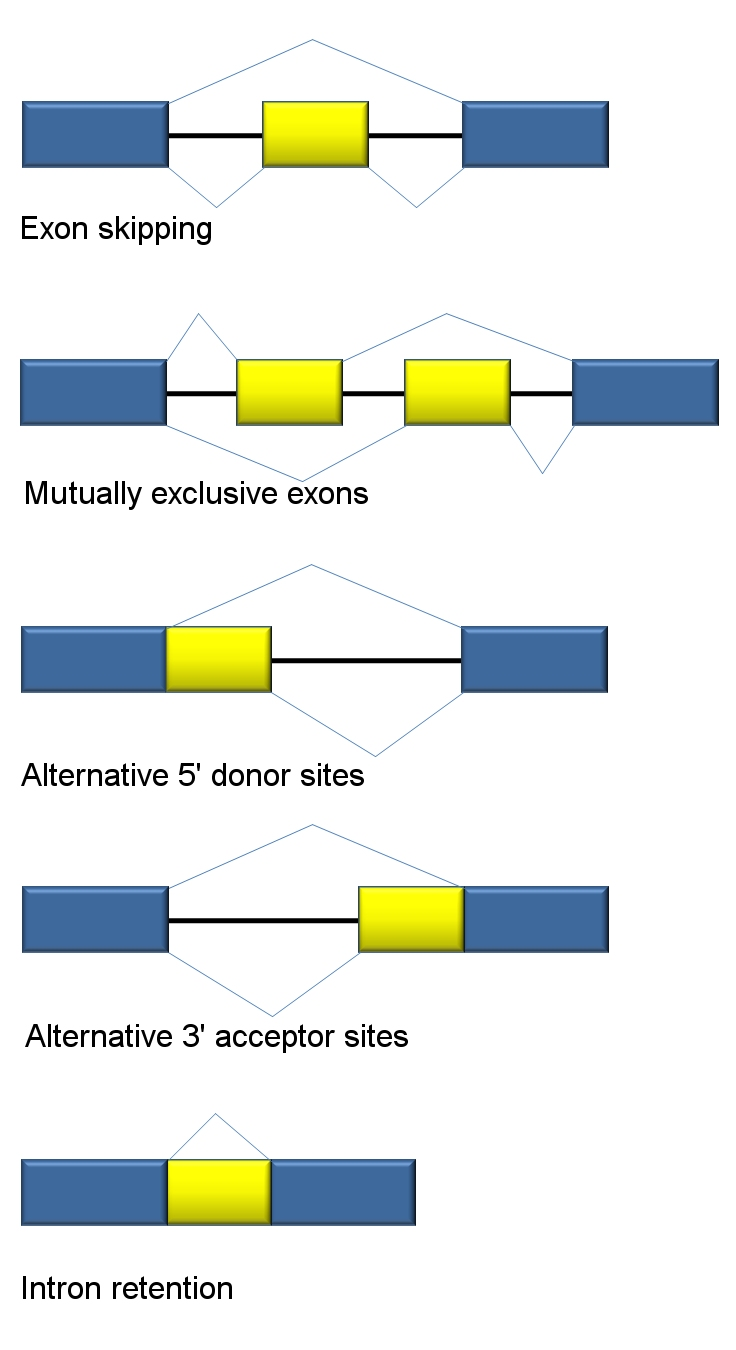
\includegraphics[height=10cm,width=10cm]{images/alternativesplicingevents.jpg}
  \caption{I diversi tipi di Alternative Splicing}
  \label{fig:AlternativeSplicingTypes}
\end{figure}